\documentclass{beamer}
% Required Packages
\usepackage{graphicx} % Required for including images
\usepackage{babel} % Required for language settings
\usepackage{listings} % Required for code listings
\usepackage{ragged2e} % Required for text justification
\usepackage{caption}
\captionsetup[figure]{name=}
\usefonttheme{professionalfonts}
%Theme and Color
\usetheme{Warsaw}
\usecolortheme{orchid}

% Font Sizes
\renewcommand{\normalsize}{\fontsize{10}{12}\selectfont}
\setbeamerfont{title}{size=\huge}
\setbeamerfont{frametitle}{size=\Large}
% Itemize Template
\setbeamertemplate{itemize items}[default]
% Title slide
\title{ACHIEVO}
\subtitle{A Productivity WebApp}
\institute[Program]{
	\inst{Women Engineers}
	\inst{TalentSprint}
}
\date{22/06/2023}
\begin{document}	
	\maketitle
	\begin{frame}{Team Members}
		\begin{itemize}
		\item Nidhi Iyer
		\item Khyati Satija
		\item Pankhuri Asthana
		\item Srinayana Mandalapu
		\item Anushka Shankar
		\end{itemize}
	\end{frame}

	

	\begin{frame}{Problem Statement}
		\justifying
		\begin{itemize}
		\item Decrease in productivity and consistency
	  \bigskip	\item Decline in attention span due to social media
		\end{itemize}
	\end{frame}

	\begin{frame}{Solution}
		\justifying
		\begin{itemize}
		\item The app increases focus levels and attention span of the user
  \bigskip
		\item It provides multiple effective productivity techniques  
		\end{itemize}
	\end{frame}

 \begin{frame}{Objectives}
                \begin{itemize}
                \item To enhance our learning.
                \item To explore various technologies via the process
                \item To gain insights into how such features work.
                \item To implement our learnings and knowledge into our web-app
                \item To deploy it and provide a solution to the raised issue
                \end{itemize}
        \end{frame}
	\begin{frame}{Description}
		\begin{itemize}
		\item The app gamifies productivity based on general human psychology
	  \bigskip	\item It includes proven methods to beat procrastination
		  \bigskip \item It includes motivational content
		\end{itemize}
	\end{frame}

	\begin{frame}{Target Audience}
	\begin{columns}
        \begin{column}{0.7\textwidth} % Adjust the width as needed
            % Content on the left side of the slide
			\begin{itemize}
			\item School and college students
  \bigskip			\item Competitive Exam Candidates
	  \bigskip		\item Working professionals of all age groups
			\end{itemize}

    	\end{column}
        
    	\begin{column}{0.3\textwidth} % Adjust the width as needed
            \begin{figure}
                
\includegraphics[width=\textwidth]{student.jpeg}
            \end{figure}
    	\end{column}
    \end{columns}
	\end{frame}

	\begin{frame}{Features}
                \begin{itemize}
		        	\item Pomodoro Technique
                	\item To-Do list (1-3-5 rule)
                	\item Eisenhower matrix
                	\item Milestone Setter
                	\item Fill the Container
                	\item Reward based point system
                	\item Productivity tracker
                \end{itemize}
        \end{frame}


	\begin{frame}{Future Additions}
	\begin{columns}
        \begin{column}{0.7\textwidth} % Adjust the width as needed
            % Content on the left side of the slide
        \begin{itemize}

		\item Group and Global Leaderboards
        \item The Motivating Spinning Wheel
        \item The Good Scroll
        \item Marathon Mode
        \item The-Hour-Rule
		\item Dilemma Bar

	\end{itemize}

    \end{column}
        
    \begin{column}{0.3\textwidth} % Adjust the width as needed
        \end{column}
	\end{columns}
	\end{frame}


	\begin{frame}{Tech Stack}
		
    \begin{figure}
        \begin{minipage}[t]{0.2\textwidth}
            \centering
            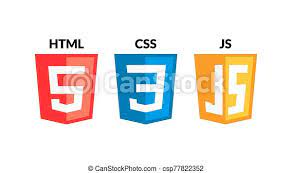
\includegraphics[width=\textwidth]{frontend.jpeg}
            \caption{Frontend}
        \end{minipage}\hfill
        \begin{minipage}[t]{0.2\textwidth}
            \centering
            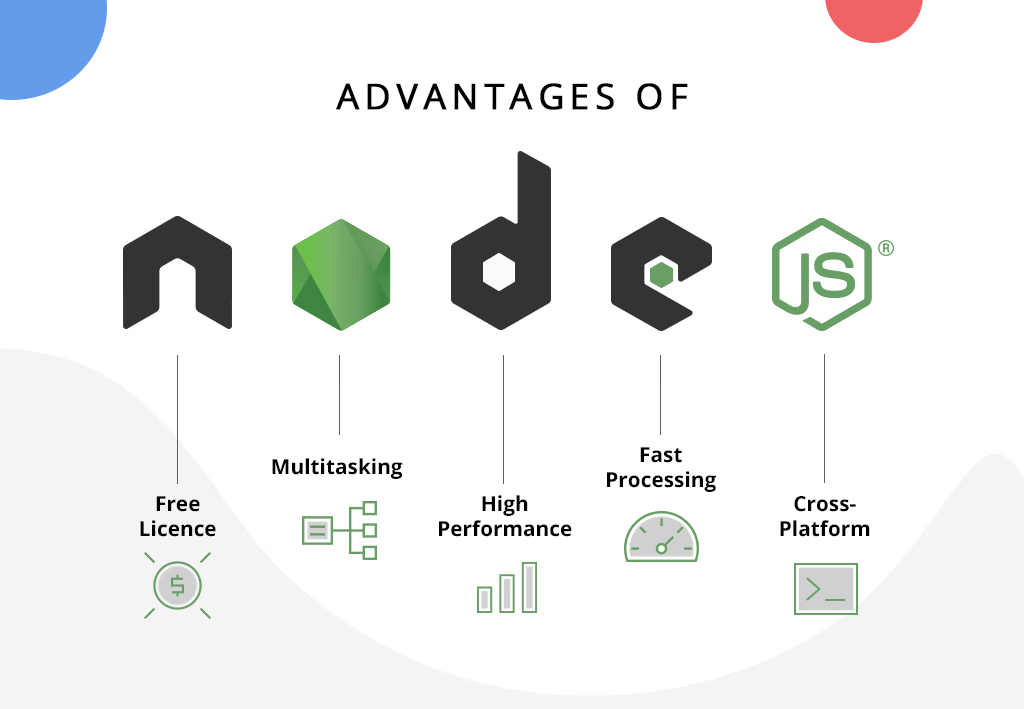
\includegraphics[width=\textwidth]{node.js_backend.png}
            \caption{Backend}
        \end{minipage}\hfill
        \begin{minipage}[t]{0.2\textwidth}
            \centering
            
\includegraphics[width=\textwidth]{mongoDB.png}
            \caption{Database}
        \end{minipage}\hfill
        \begin{minipage}[t]{0.2\textwidth}
            \centering
            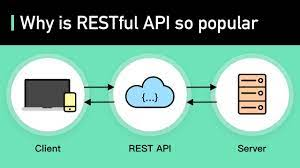
\includegraphics[width=\textwidth]{API.jpeg}
            \caption{RESTful APIs}
        \end{minipage}\hfill
    \end{figure}
	\end{frame}

 \begin{frame}{Work Done}
                \justifying
                \begin{itemize}
                \item  Created Git Repository
                \item  Decided the tech stack
                \item  Made Weekly Plans and set milestones
                \item  Discussed a rough idea of visual frame-work
                \item  Learnt Sphinx for docs
                \item Improved the \LaTeX{} presentation
                \item  Started learning HTML
                \item  Researched about APIs and cloud platforms
                \end{itemize}
        \end{frame}
	% \begin{frame}{USP}
	% 	\justifying
	% 	Unique Selling Proposition:
	% 	\begin{itemize}
	% 	\item Unmatched range of productivity features
	% 	\item Utilizes user statistics for performance comparison
	% 	\item Multiple productivity features		
	% 	\item Gamification of the work by leveraging reward based human psychology
		
	% 	\end{itemize}
	% \end{frame}

	

	\begin{frame}{Conclusion}
		\justifying
		Hence, Let's ACHIEVO \\ 
 \bigskip
		\textbf{Domain: } Web Development \\
		\textbf{Status: } Ideation \\
		
		\bigskip
		
		\Huge\textbf{Thank You !}
	\end{frame}

\end{document}
